% EMQ Stabilization Presentation (15‑minute)
\documentclass[aspectratio=169]{beamer}
\usetheme{Madrid}
\usepackage[utf8]{inputenc}
\usepackage{graphicx}
\usepackage{booktabs}
\usepackage{xcolor}
\usepackage[linesnumbered,ruled,vlined]{algorithm2e}
\title[Stabilizing EM‑Based Quantification]{Stabilizing EM‑Based Quantification under Label Shift}
\author{Pablo González, Olaya Pérez-Mon, Juan José del Coz}
\institute[AI Center, Uni. Oviedo]{Artificial Intelligence Center\\University of Oviedo}
\date{LQ 2025 · September 15, 2025}

\begin{document}

%---------------------------------------------------------
\begin{frame}
  \titlepage
\end{frame}

%---------------------------------------------------------
\begin{frame}{Motivation}
  \begin{itemize}
    \item \alert{Quantification goal}: estimate \textbf{class prevalences} in an \emph{unlabelled} target sample.
    \item \textbf{Assumptions} for most quantification methods:
          \begin{itemize}
            \item \textbf{Prior probability shift}: $P(X\mid Y)=Q(X\mid Y)$ while $P(Y)\neq Q(Y)$.
            %\item \textbf{Well‑calibrated posteriors}: we can obtain reliable estimates of $p(y\mid x)$ from a source classifier.
          \end{itemize}
    \item Under these conditions,  \textbf{EMQ}
          \begin{itemize}
            \item coincides with the maximum‑likelihood estimator,
            \item is \emph{Fisher‑consistent}: perfect estimation as the sample size grows,
            \item fast and a very strong baseline for quantification problems.
          \end{itemize}
    \item Yet, in practical problems, mild violations of the assumptions (e.g.\ mis‑calibration of the underlying classifier) can lead to oscillations and degenerate estimates $\Rightarrow$ motivation for stabilization.
  \end{itemize}
\end{frame}

%---------------------------------------------------------
\begin{frame}{Baseline: EMQ}
  EM is an iterative algorithm that uses Bayes’ rule to estimate the target class distribution $Q(c)$ by alternating between two steps:
  
  \begin{itemize}
    \item $Q(c)$: Prevalence of class $c$ in the target set.
    \item $P(c)$: Prevalence of class $c$ in the training set.
    \item $s_i(c)$: Score (e.g., soft prediction) assigned to class $c$ by the classifier for instance $i$.
    \item $q_i^{(t)}(c)$: Estimated probability that instance $i$ belongs to class $c$ at iteration $t$.
  \end{itemize}

  \begin{columns}
    \begin{column}{0.4\textwidth}
      \begin{block}{E‑step (Expectation)}
        \small
        Update instance-level posteriors:
        $$q_i^{(t)}(c)=\frac{\frac{Q^{(t)}(c)}{P(c)}\,s_i(c)}{\sum_{j=1}^{K}\frac{Q^{(t)}(j)}{P(j)}\,s_i(j)}$$
      \end{block}
    \end{column}
    \begin{column}{0.4\textwidth}
      \begin{block}{M‑step (Maximization)}
        \small
        Update class prevalences:
        $$Q^{(t+1)}(c)=\frac{1}{N}\sum_{i=1}^{N}q_i^{(t)}(c)$$
      \end{block}
    \end{column}
  \end{columns}
\end{frame}


%---------------------------------------------------------
\begin{frame}{Practical Limitations of EMQ}
  Although EMQ is a theoretically sound and widely adopted baseline, its practical performance is often mixed, especially in real-world settings:

  \begin{itemize}
    \item Highly sensitive to \textbf{mis‑calibrated} posteriors.
    \item Tends to produce \textbf{degenerate estimates} when some classes are rare in the test distribution.
    \item In the \textbf{multiclass} setting, errors can propagate and compound across classes.
    \item \textbf{Empirical studies} in the literature report strong performance in some datasets, but also significant failures in others (even when a good calibrator is used).
  \end{itemize}
\end{frame}


%---------------------------------------------------------
\begin{frame}{Our Contributions}
  \begin{enumerate}
    \item \textbf{Unified Framework}: Decompose EMQ into two modular components:
          \begin{itemize}
            \item E-step: \textit{Posterior Transformation} $\mathcal{C}$
            \item M-step: \textit{Prevalence Update} $\mathcal{U}$
          \end{itemize}
    \item Systematic taxonomy of existing \& novel stabilisation heuristics (both for the E-step and the M-step).
    \item Exhaustive evaluation on 20+ UCI datasets.
  \end{enumerate}
\end{frame}

%---------------------------------------------------------
\begin{frame}[fragile]{Unified EMQ Framework}
\fontsize{8.5}{8.5}\selectfont
\begin{algorithm}[H]
\DontPrintSemicolon
\SetAlgoNoLine % optional: removes vertical lines
\SetNlSty{}{\color{gray}}{} % makes line numbers subtle (optional)
\KwIn{Unlabeled instances $\mathcal{D}_T = \{x_1, \ldots, x_n\}$, classifier posteriors $s_i(c)$, \textcolor{red}{posterior transformation} $\mathcal{C}$, \textcolor{red}{update function} $\mathcal{U}$}
\KwOut{Estimated target class prevalences $Q(Y)$}
Initialize prevalence estimate $Q^{(0)} \in \Delta^K$\;
\Repeat{convergence}{
  \ForEach{instance $x_i \in \mathcal{D}_T$}{
    
    Compute reweighted posterior: \\
    $q^{(t)}_i(c) \gets \dfrac{\frac{Q^{(t)}(c)}{P(c)} \cdot s_i(c)}{\sum_{j=1}^K \frac{Q^{(t)}(j)}{P(j)} \cdot s_i(j)}$\;
    Apply reweighted posterior transformation: \\
    $\tilde{q}^{(t)}_i \gets \textcolor{red}{\mathcal{C}}\!\big(q^{(t)}_i\big)$\;
    }
  Compute raw prevalence update: \\
  $\hat{Q}^{(t+1)}(c) \gets \dfrac{1}{N} \sum_{i=1}^N \tilde{q}^{(t)}_i(c)$\;
  Update prevalence estimate: \\
 $Q^{(t+1)} \gets \textcolor{red}{\mathcal{U}}\!\bigl(Q^{(t)},\, \hat{Q}^{(t+1)},\, \{\tilde{q}^{(t)}_i\}_{i=1}^N\bigr)$\;
}
\Return $Q^{(t+1)}$\;
\caption{Unified EMQ Framework}
\end{algorithm}
\end{frame}


%---------------------------------------------------------
\begin{frame}{E‑Step Heuristics ($\mathcal{C}$)}
  \begin{itemize}
    \item \textbf{Calibration (BCTS)}: Applies a post-processing transformation to classifier scores to improve reliability.\\
    \small Used only once before EM begins and helps align $s_i(c)$ with true posteriors (not part of the framework).
    \normalsize

    \item \textbf{Posterior Smoothing}: $\tilde{q}_i^{(t)}(c)\! \leftarrow\! ({q}_i^{(t)}(c)+\varepsilon)/(1+K\cdot\varepsilon)$\\
    \small Prevents zero probabilities and softens overconfident predictions, especially useful when some classes are rare or underrepresented.
    \normalsize

    \item \textbf{Temperature Scaling}: $\tilde{q}_i^{(t)}(c) \leftarrow q_i^{(t)}(c)^{1/\tau}$ then renormalize\\
    \small Dynamically flattens (or sharpens) the score distribution during EM. 
    \small Applies a power transformation to soften or sharpen posteriors during EM:\\
    - \( \tau > 1 \): flattens the distribution, reducing overconfidence.\\
    - \( \tau < 1 \): sharpens the distribution, making predictions more confident.\\Helps mitigate overconfident predictions and stabilizes updates.
  \end{itemize}
\end{frame}


%---------------------------------------------------------
% REVISAR NOTACIÓN%
\begin{frame}{M‑Step Heuristics ($\mathcal{U}$)}
  \begin{itemize}
    \item \textbf{MAP / Dirichlet Prior}: Add $\alpha$-1 pseudo-counts to the prevalence update $Q^{(t+1)}(c) = \frac{\sum_{i=1}^N \tilde{q}_i^{(t)}(c) + \alpha - 1}{N + K(\alpha - 1)}$.
    When $\alpha>1$, the prevalence updates are pulled towards the uniform distribution. 

    \item \textbf{Damping}: Blend the new estimate with the previous one $Q^{(t+1)} \gets (1-\lambda) Q^{(t)} + \lambda \hat{Q}^{(t+1)}$   \\
    
    \small Slows down updates to avoid abrupt changes; effective for noisy or unstable posteriors.
    \normalsize

    \item \textbf{Confidence Selection}: Use only the most confident instances to compute $Q^{(t+1)}$.\\
    \small Reduces the influence of uncertain predictions, filtering top-$\kappa$ instances with highest max-score.
    \normalsize

    \item \textbf{Entropy Regularization}: Encourages high-entropy (i.e., smoother) prevalence vectors:\\
    \[
        \arg\max_Q \sum_{c=1}^K \hat{Q}(c) \log Q(c) + \eta H(Q)
    \]
    \small Acts as a regularizer to prevent overconfident or peaked estimates. $\eta$ controls the strength of the penalty.
  \end{itemize}
\end{frame}


%---------------------------------------------------------
\begin{frame}{Experimental Setup}
  \begin{itemize}
    \item \textbf{Datasets}: 24 multiclass UCI datasets, test bags = 1000 (per dataset), bag size = 500.
    \item \textbf{Metric}: Mean Absolute Error (MAE).
    \item \textbf{Hyper‑parameters}: tuned on validation bags via \textit{QuaPy} along with the classifier hyperparameters.
  \end{itemize}
  \centering
  \begin{table}[h]
\centering
\label{tab:hyperparams}
\begin{tabular}{ll}
Heuristic & Hyperparameter range\\
\hline
 \textit{Smooth} & $\epsilon \in \{\textbf{0}, 10^{-6}, 10^{-5}, 10^{-4}\}$ \\
\textit{Temp}   & $\tau \in \{0.25, 0.5, 0.75, \textbf{1.0}, 1.25, 1.5, 2.0, 3.0, 5.0\}$ \\
 \textit{Damp}   & $\lambda \in \{0.1, 0.2, \ldots, \textbf{1.0}\}$ \\
 \textit{Ent}    & $\eta \in \{\textbf{0.0}, 0.0001, 0.001\}$ \\
\textit{MAP}    & $\alpha \in \{\textbf{1.0}, 2.0, 5.0, 10.0\}$ \\
\textit{Conf}   & $\kappa \in \{0.3, 0.5, 0.8, \textbf{1.0}\}$ \\
\hline
\end{tabular}
\end{table}
\end{frame}


%---------------------------------------------------------
\begin{frame}{Overall Results}
  \centering
  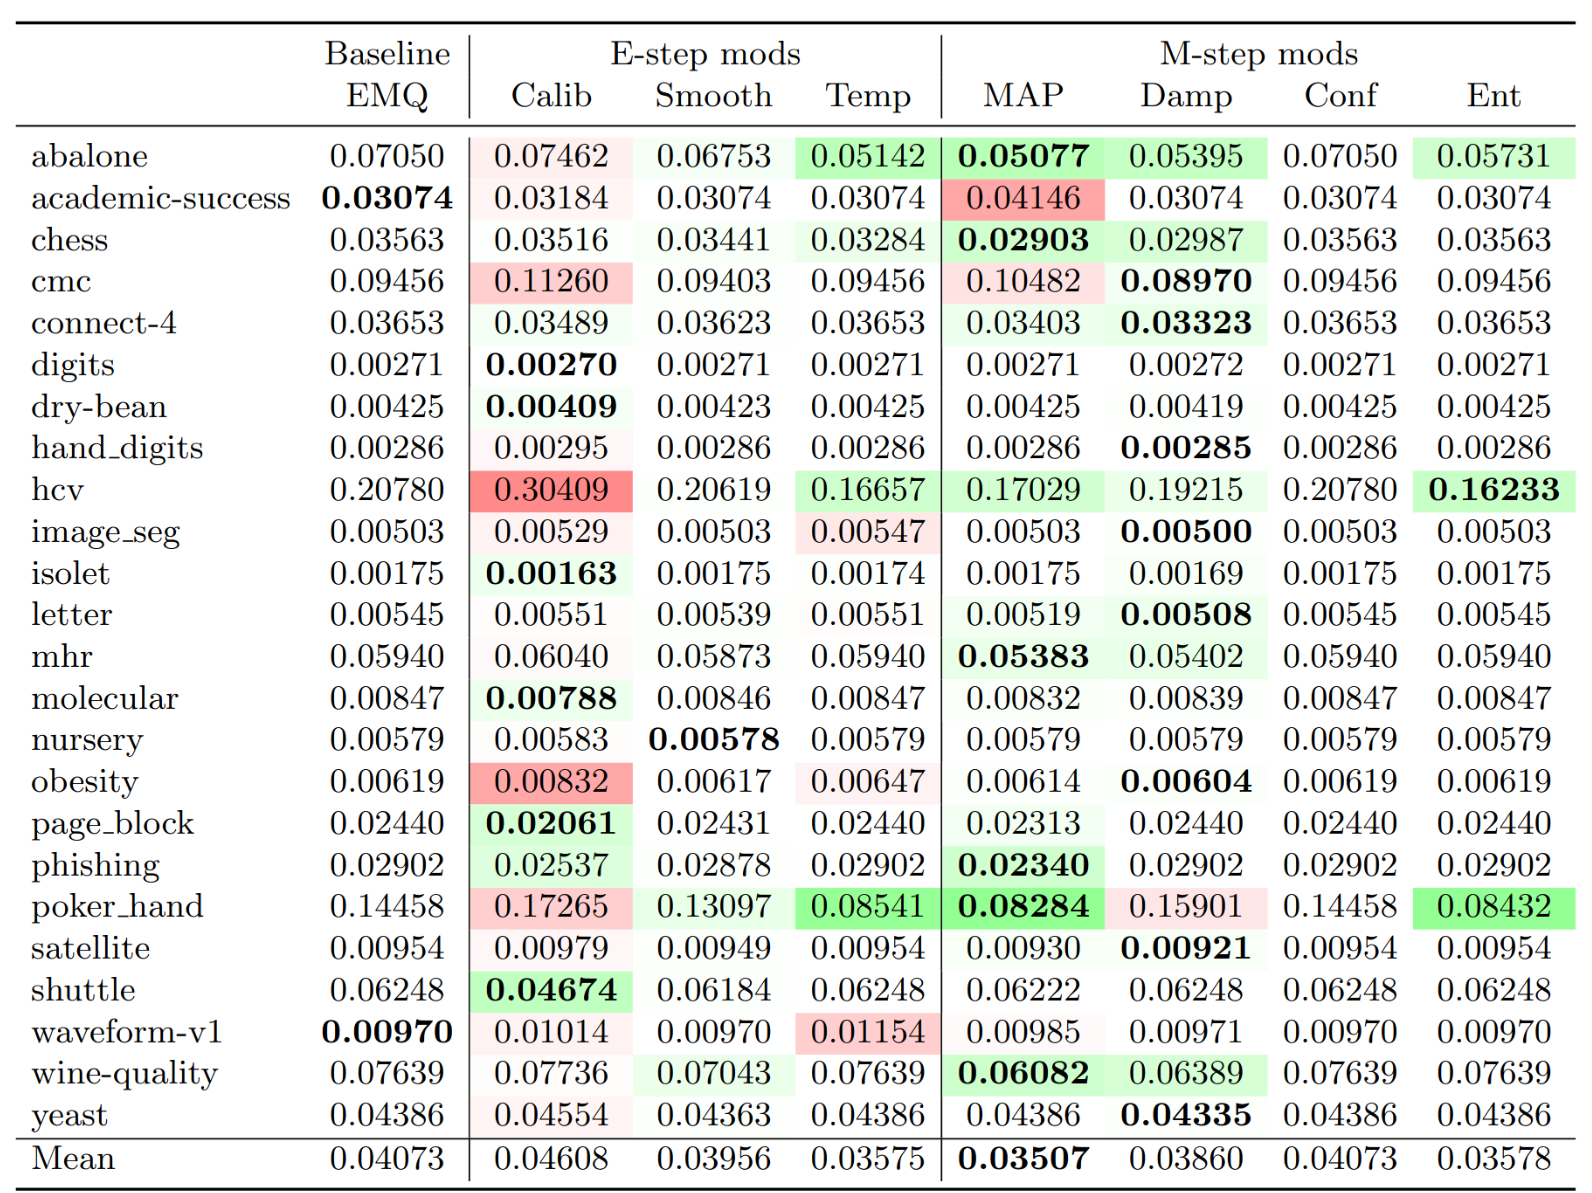
\includegraphics[width=0.6\linewidth]{images/results_lr.png}
\end{frame}


\begin{frame}{Bag-level: statistical analysis}
  \centering
  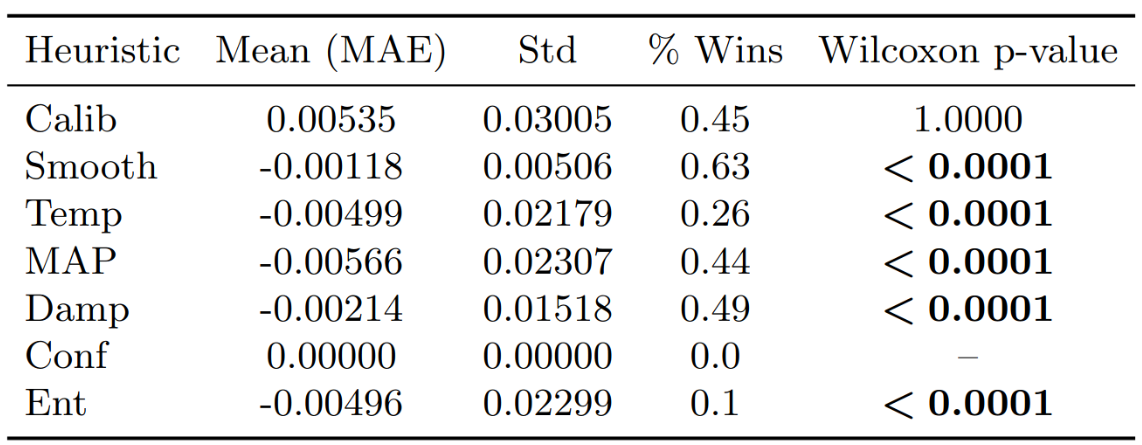
\includegraphics[width=0.6\linewidth]{images/statistical_analysis.png}
\end{frame}

\begin{frame}{Dataset level: Win-ties-losses charts}
  \centering
    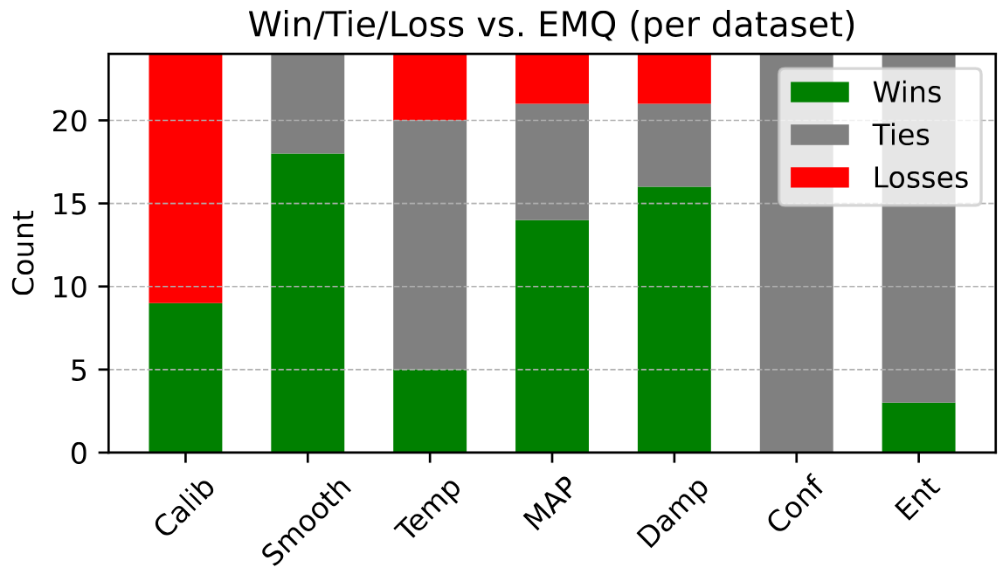
\includegraphics[width=0.6\linewidth]{images/datasetlevel.png}
\end{frame}

\begin{frame}{Combinating heuristics}
  \centering
    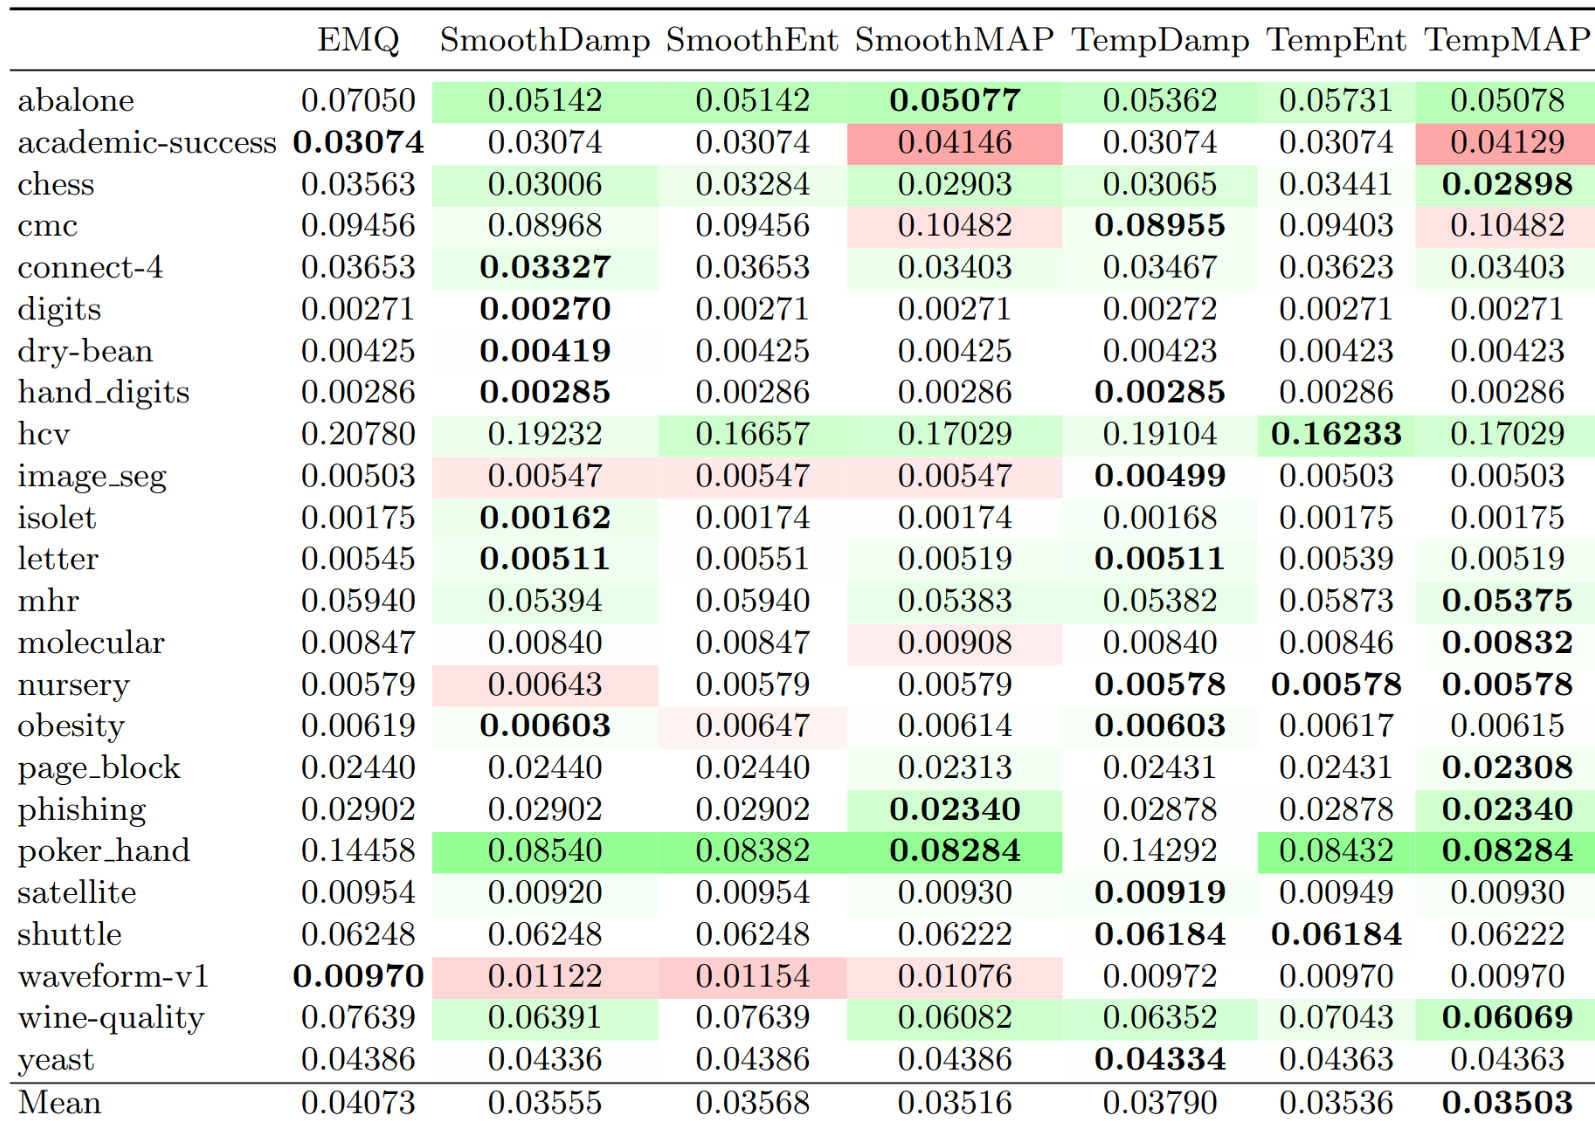
\includegraphics[width=0.6\linewidth]{images/combinations.png}
\end{frame}

%---------------------------------------------------------
\begin{frame}{Key Insights}
  \begin{itemize}
    \item \textbf{Dataset specific}: even though some heuristics like \textit{Entropy regularization} or \textit{MAP} show some pretty consistent results, they should be considered based on the data.
    \item \textbf{Modularity}: heuristics can fall back to plain EMQ, using a grid search to enable automatic selection.
    \item \textbf{Proposed framework}: it allows the design of new heuristics by combining existing ones, e.g., \textit{Smooth + MAP} or \textit{Temp + Entropy}.
  \end{itemize}
\end{frame}

%---------------------------------------------------------
\begin{frame}{Conclusions and Future work}
  \begin{itemize}
    \item We presented a \textbf{unified framework} + extensive heuristic benchmarking.
    \item Simple heuristics can yield significant improvements over standard EMQ.
    \item Heuristic are lightweight, easy to implement and pretty safe to use.
    \item Future work
    \begin{itemize} 
      \item explore automatic selection of heuristics.
      \item derive consistency guarantees.
      \item explore heuristics for other types of shifts or situations where basic EMQ might fail.
    \end{itemize}
  \end{itemize}
\end{frame}

%---------------------------------------------------------
\begin{frame}
  \centering
  \Huge
Questions?
\\ 
\vspace{1cm}

\includegraphics[width=0.6\textwidth]{images/questions.png}
\end{frame}

\end{document}